\documentclass[a4paper,12pt, italian]{article}
\usepackage{geometry}
\geometry{a4paper, top=3cm, bottom=3cm, left=3cm, right=3cm, heightrounded, bindingoffset=5mm}
\usepackage[italian]{babel}
\usepackage[version=3]{mhchem} 
\usepackage{siunitx} 
\usepackage{graphicx}
\usepackage{booktabs}
\usepackage{natbib} 
\usepackage{amsmath}
\usepackage{hyperref}
%\usepackage[labelformat=empty]{caption}
\setlength\parindent{15pt}
\usepackage{natbib}
\usepackage{amscd}
\usepackage{siunitx}
\usepackage{booktabs}
\usepackage{multicol}
\usepackage{tikz}
\usepackage{amsmath,amssymb}
\usepackage{amsthm}
\usepackage{tikz}
\usepackage{cancel}
\usepackage{placeins} %aggiungi questo package e usa \FloatBarrier all'inizio e alla fine della sequenza di tabelle
\usepackage[labelsep=space]{caption} 
\renewcommand{\labelenumi}{\alph{enumi}.} 
\newcommand{\minitab}[2][l]{\begin{tabular}#1 #2\end{tabular}}

\title{\textsc{Studio delle leggi che governano le inteterferenze con sorgenti nello spettro delle microonde}}
\date{}

\author{Laura \textsc{Trombetta}\\ Alessandro Maria \textsc{Turturiello}\\Federico \textsc{Venturoli}} 



\begin{document}

\maketitle 

\begin{center}
\begin{tabular}{l r}
Eseguita il giorno: &  31 marzo 2022 \\ 
Gruppo T2A-4: & Trombetta Laura\\
& Turturiello Alessandro Maria \\
& Venturoli Federico \\ 

\end{tabular}
\end{center}
\begin{abstract}
    Lo scopo della relazione è lo studio delle leggi dell'ottica, grazie all'utilizzo di un'onda elettromagnetica che rientra nel range delle microonde.
    Abbiamo condotto molteplici esperimenti per verificare le leggi di polarizzazione, riflessione, rifrazione, interferenza e la natura stazionaria dell'onda in specifiche condizioni. Gli esperimenti hanno avuto nel complesso risultati soddisfacenti, in caso contrario siamo riusciti ad identificare la sorgente dell'errore, in modo da non invalidare la legge che stavamo verificando. 
\end{abstract}
\tableofcontents
\maketitle
\newpage

\section{Introduzione e descrizione dell'apparato sperimentale}
Per condurre l'esperienza ci siamo serviti di una Breadboard dotata di due boccole e di una griglia di fori in cui inserire i refori. La griglia è caratterizzata dalla presenza di quattro colonne indicate con i simboli "+" e "-", ciascuna equipotenziale, e altre venti colonne equipotenziali riga per riga, indicate con delle lettere. Lo strumento ci ha permesso di realizzare i circuiti su cui abbiamo condotto le diverse misure. Le componenti di circuito di cui ci siamo serviti sono state le resistenze, di cui abbiamo ricavato i valori tramite un \textit{tool online}\footnote{ https://www.digikey.it/it/resources/conversion-calculators/conversion-calculator-resistor-color-code}, diodi di silicio e un partitore resistivo, composto da boccole e da interruttori in grado di modificare la resistenza dello strumento.
Abbiamo fatto uso di due multimetri, strumenti in grado di misurare diverse grandezze, nel nostro caso utilizzati per determinare la differenza di potenziale tra due punti del circuito e l'intensità di corrente.
Infine, abbiamo collegato un generatore che fornisse corrente ai circuiti, attraverso il controllo della sua differenza di potenziale.

\begin{figure}[h!]
    \centering
    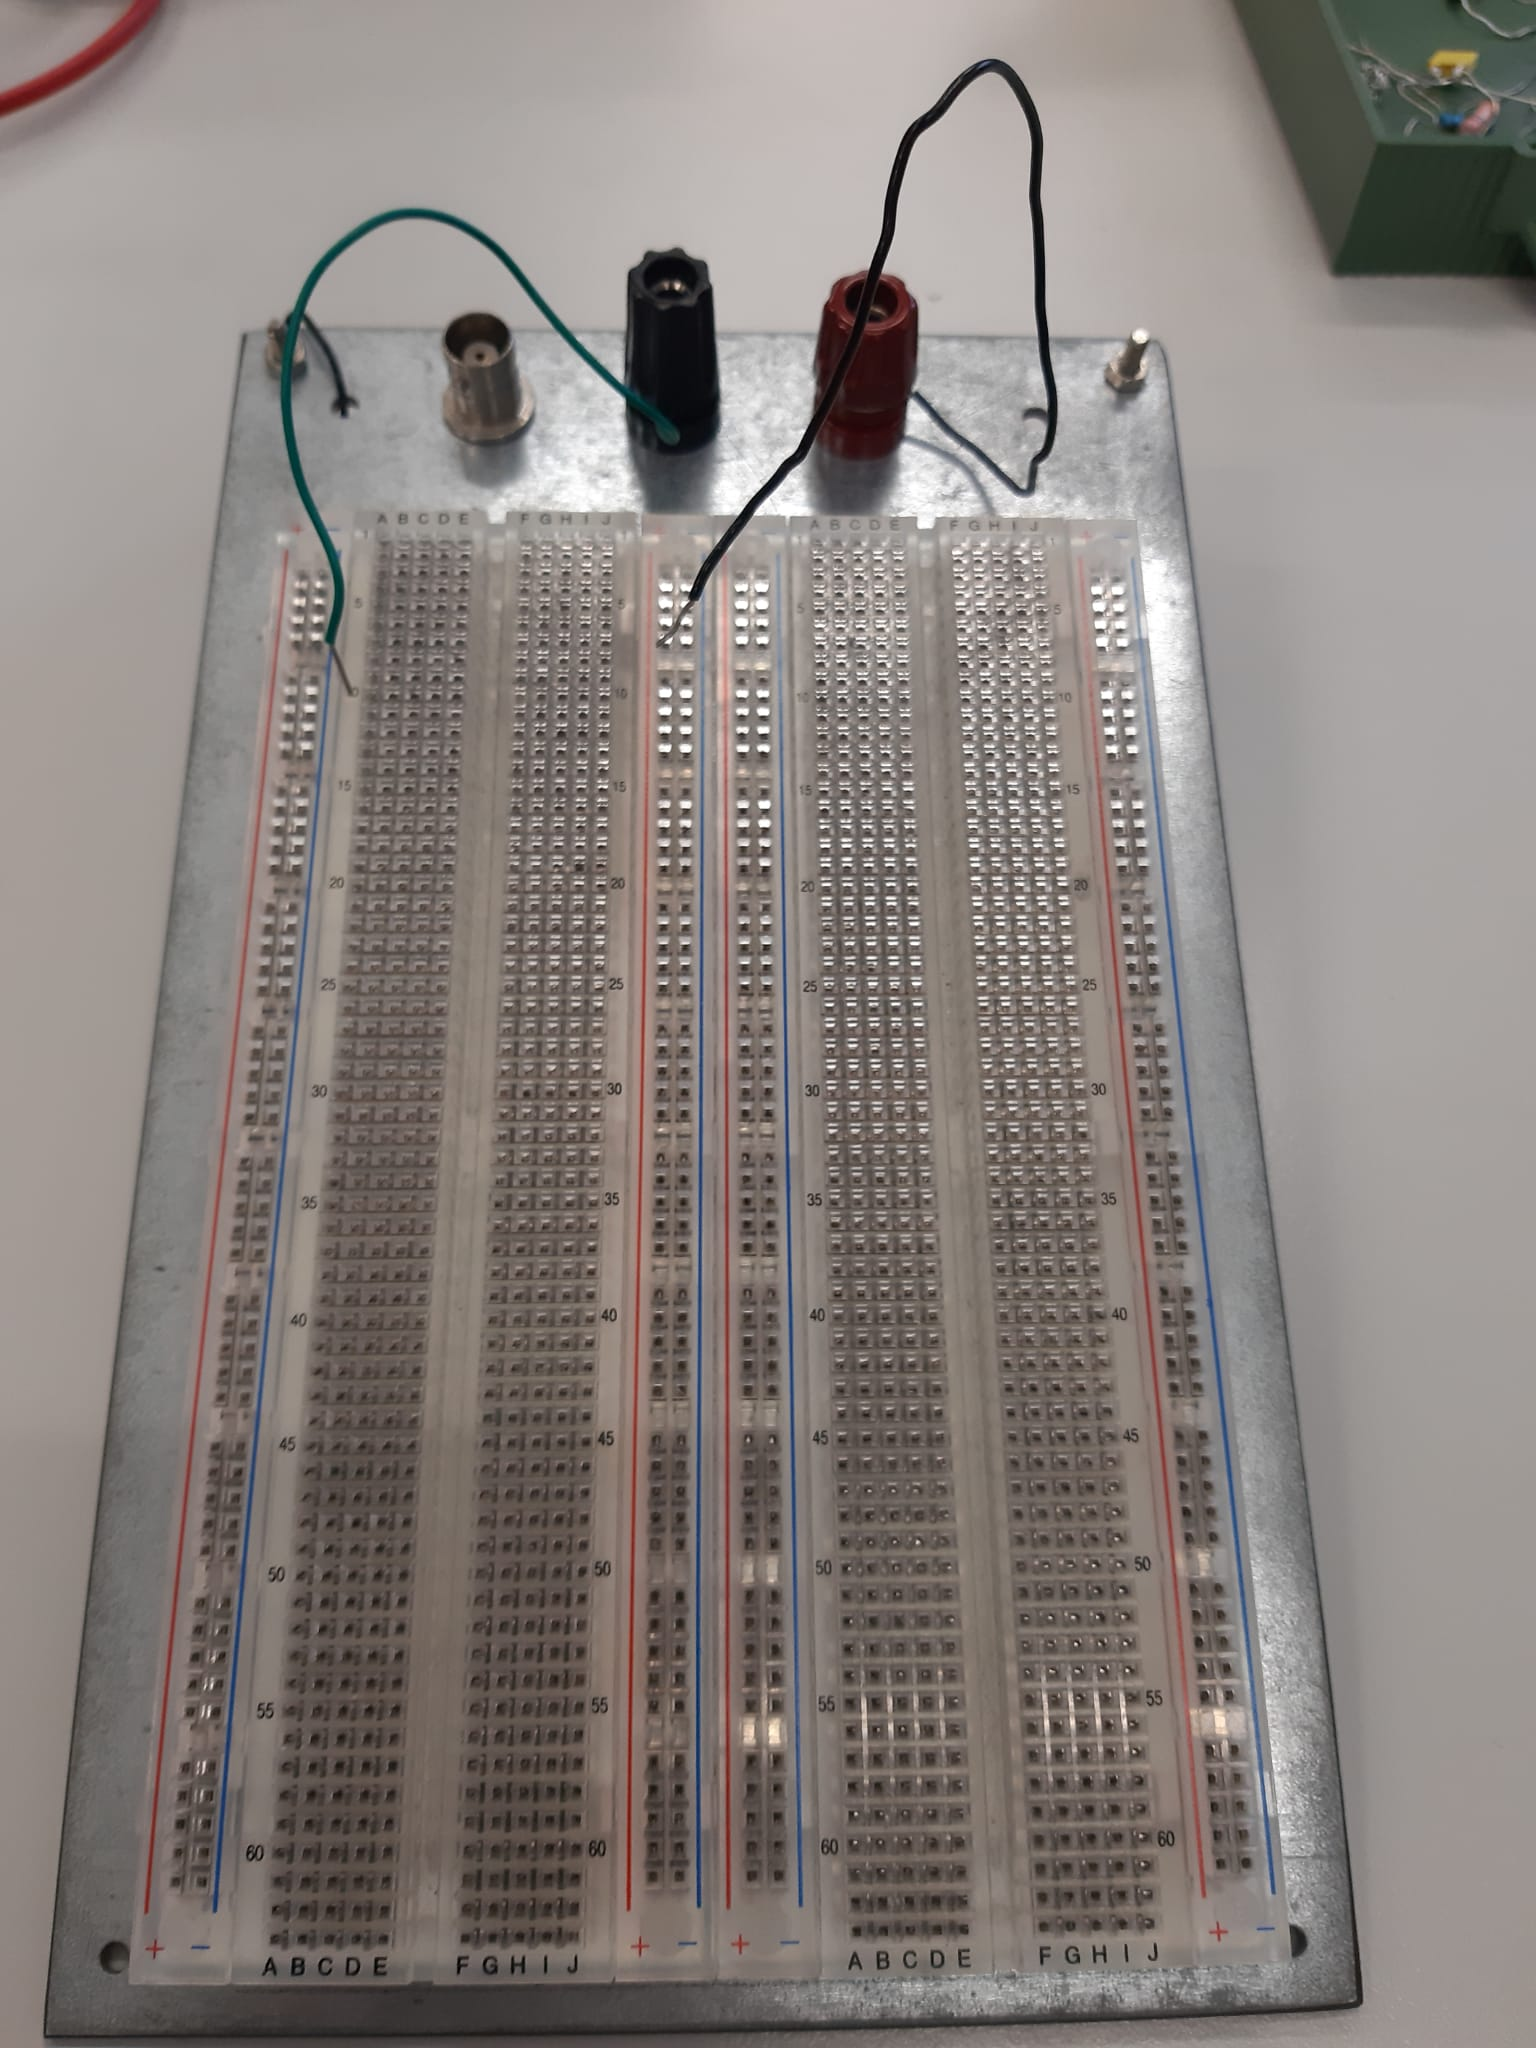
\includegraphics[scale=0.1]{Immagini/Circuitoooo.jpeg}
    \label{fig:my_label}
\end{figure}

La prima parte dell'esperienza si è concentrata sullo studio della strumentazione di laboratorio, studio finalizzato ad utilizzare configurazioni adeguate nelle parti successive. E' stato, infatti, necessario verificare che il multimetro usato come Voltmetro fosse ben progettato, cioè che avesse la caratteristica di possedere una resistenza in parallelo grande. Analogamente, è stato necessario verificare che il multimetro usato come Amperometro avesse la caratteristica di possedere una resistenza in serie piccola.
Successiavmente ci siamo concenrati sullo studio delle resistenze e della Legge di Ohm:

\begin{equation}
\frac{1}{R_{\parallel}}=\sum_{i=1}^{N}\frac{1}{R_{i}} \hspace{73 pt} R_{\perp}=\sum_{i=1}^{N}R_{i}
\end{equation}

\begin{equation}
V=R_{tot}I
\end{equation}

Infine, abbiamo studiato la Legge di Shockley, che descrive l'andamento di corrente per i diodi:

\begin{equation}
I=I_{0}(e^{qv/gK_b T}-1)
\end{equation}

indicando con \textit{q} la carica degli elettroni, con $K_b$ la costante di Boltzmann, con \textit{g} la costante che dipende dal tipo di diodo e con T la temperatura del diodo in Kelvin, corrispondente a quella dell'ambiente. Il termine di proporzionalità $I_0$ è detto \textit{intensità di corrente di saturazione}, il valore che ci aspettiamo di ottenere è molto piccolo in quanto si tratta di una corrente generata dai portatori di carica interni al diodo in diffusione dalla regione neutra alla regione di carica spaziale\footnote{Si tratta di una regione isolante all'interno di un semiconduttore drogato.}.
\section{Onde stazionarie}
Obiettivo di questa sezione è stato quello di misurare la lunghezza d'onda $\lambda $ di una microonda, il cui range di grandezza varia tra 1 mm e 30 cm.

Abbiamo preferito procedere contando il numero di massimi, corrispondenti al punto di inversione della lancetta dell'amperometro, per una lunghezza di d = 20 cm. Questa scelta è stata motivata dal fatto che preferire, invece, un passo piccolo avrebbe aumentato l'imprecisione. Quest'ultima è dovuta alla presenza di componenti sinusoidali aggiuntive che sporcano l'onda non perfettamente stazionaria.

Per ricavare il valore della lunghezza d'onda ci siamo serviti della relazione 
\begin{equation}
    \lambda = \dfrac{2\, d}{\text{Numero di massimi}}
\end{equation}
di seguito abbiamo riportato le lunghezze d'onda calcolate e il relativo errore ricavato dalla propagazione degli errori.

\begin{table}[h!]
    \centering
    \begin{tabular}{ccc}
        Numero massimi & $\lambda$ (cm) & errore $\lambda$\\
        \hline
    14&	2,857&	0,014\\
    13&	3,077&	0,015\\
    14&	2,857&	0,014\\
    14&	2,857&	0,014\\
    13&	3,077&	0,015\\
    13&	3,077&	0,015\\
    14&	2,857&	0,014\\
    14&	2,857&	0,014\\
    14&	2,857&	0,014\\
    14&	2,857&	0,014\\
    14&	2,857&	0,014\\
    14&	2,857&	0,014\\
    14&	2,857&	0,014\\
    14&	2,857&	0,014\\
    14&	2,857&	0,014\\
    14&	2,857&	0,014\\
\hline\hline
    \end{tabular}
    \caption{}
    \label{lunghezze donda}
\end{table}
\noindent
Il valore ottenuto è di 
$$
\lambda = (2,898 \pm 0,014)\,cm
$$
il cui errore è ricavato dalla media dei singoli errori.

\section{Riflessione e rifrazione}
\subsection{Riflessione}
Per analizzare il fenomeno della riflessione abbiamo verificato la legge di Cartesio (riportata sotto), misurando gli angoli di incidenza e riflessione della microonda su uno specchio riflettente.
\begin{equation}
    \theta_i=\theta_r
\end{equation}
\noindent
Gli angoli ricavati, misurati in gradi, sono i seguenti:

\begin{table}[h!]
    \centering
    \begin{tabular}{cccc}
    $\theta_i \, (^\circ)$ && \,$\theta_r \, (^\circ)$&\\
    \toprule
    20	&20	&&21\\
    20	&21	&&23\\
    30	&31	&&31\\
    30	&29	&&27\\
    40	&37	&&35\\
    40	&35	&&39\\
    50	&43	&&48\\
    50	&44	&&43\\
    60	&65	&&69\\
    60	&63	&&63\\
    \bottomrule
    \end{tabular}
    \caption{}
    \label{}
\end{table}

Abbiamo osservato che per angoli piccoli l'errore era maggiore, supponendo che ciò fosse dovuto al fatto che emettitore e ricevitore si trovassero troppo allineati. Probabilmente il ricevitore captava il segnale non solo dell'onda riflessa ma anche di quella emessa.
\subsection{Rifrazione}
Abbiamo studiato il fenomeno della rifrazione con lo scopo di misurare l'indice di rifrazione dello styrene, un idrocarburo aromatico.
Abbiamo posizionato un contenitore di polistirolo a base triangolare sulla pedana al centro. Dopo aver verificato che l'indice di rifrazione del polistirolo fosse pari a quello dell'aria abbiamo misurato l'angolo tra l'ipotenusa e il cateto maggiore attraverso le formule trigonometriche, l'angolo risultava essere di $\theta_v = 22,54 ^\circ$.

\begin{figure}[h!]
    \centering
    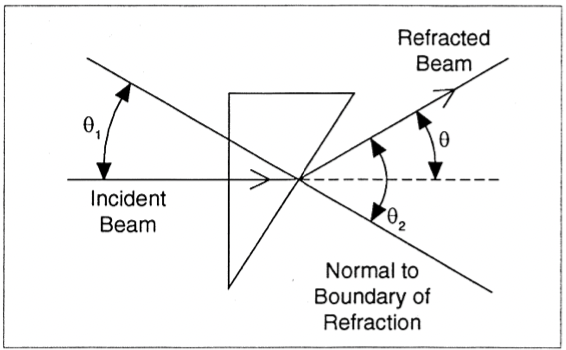
\includegraphics[scale=.7]{Immagini/triangolo.png}
    \caption{}
    \label{triangolo}
\end{figure}
 
In seguito abbiamo preso l'angolo formato con la normale, $\theta_n = 38,54 ^\circ$, da cui abbiamo ricavato il valore di n = 1,63 come indice di rifrazione dello styrene. Quest'ultimo è stato calcolato attraverso la seguente relazione:
$$
n=\dfrac{\sin\theta_n}{\sin\theta_v}
$$

\section{Polarizzazione}
Questa sezione ha come obiettivo quello di determinare la relazione tra intensità e angolo di polarizzazione.
Per condurre questa esperienza abbiamo disposto emettitore e ricevitore allineati e abbiamo ruotato il ricevitore di diversi angoli $\theta$.
Tenendo conto dell'imprecisione messa in evidenza nell'introduzione, abbiamo deciso di rappresentare la relazione in due modi differenti.
In primo luogo abbiamo utilizzato un'interpolazione lineare sul $\cos^2\vartheta$, verificando che l'apparato non avesse errore di calibrazione in base al verso della rotazione. I risultati sono riportati nella Figura \ref{polatizzazione fit quadratico}.
\begin{figure}[h!]
    \centering
    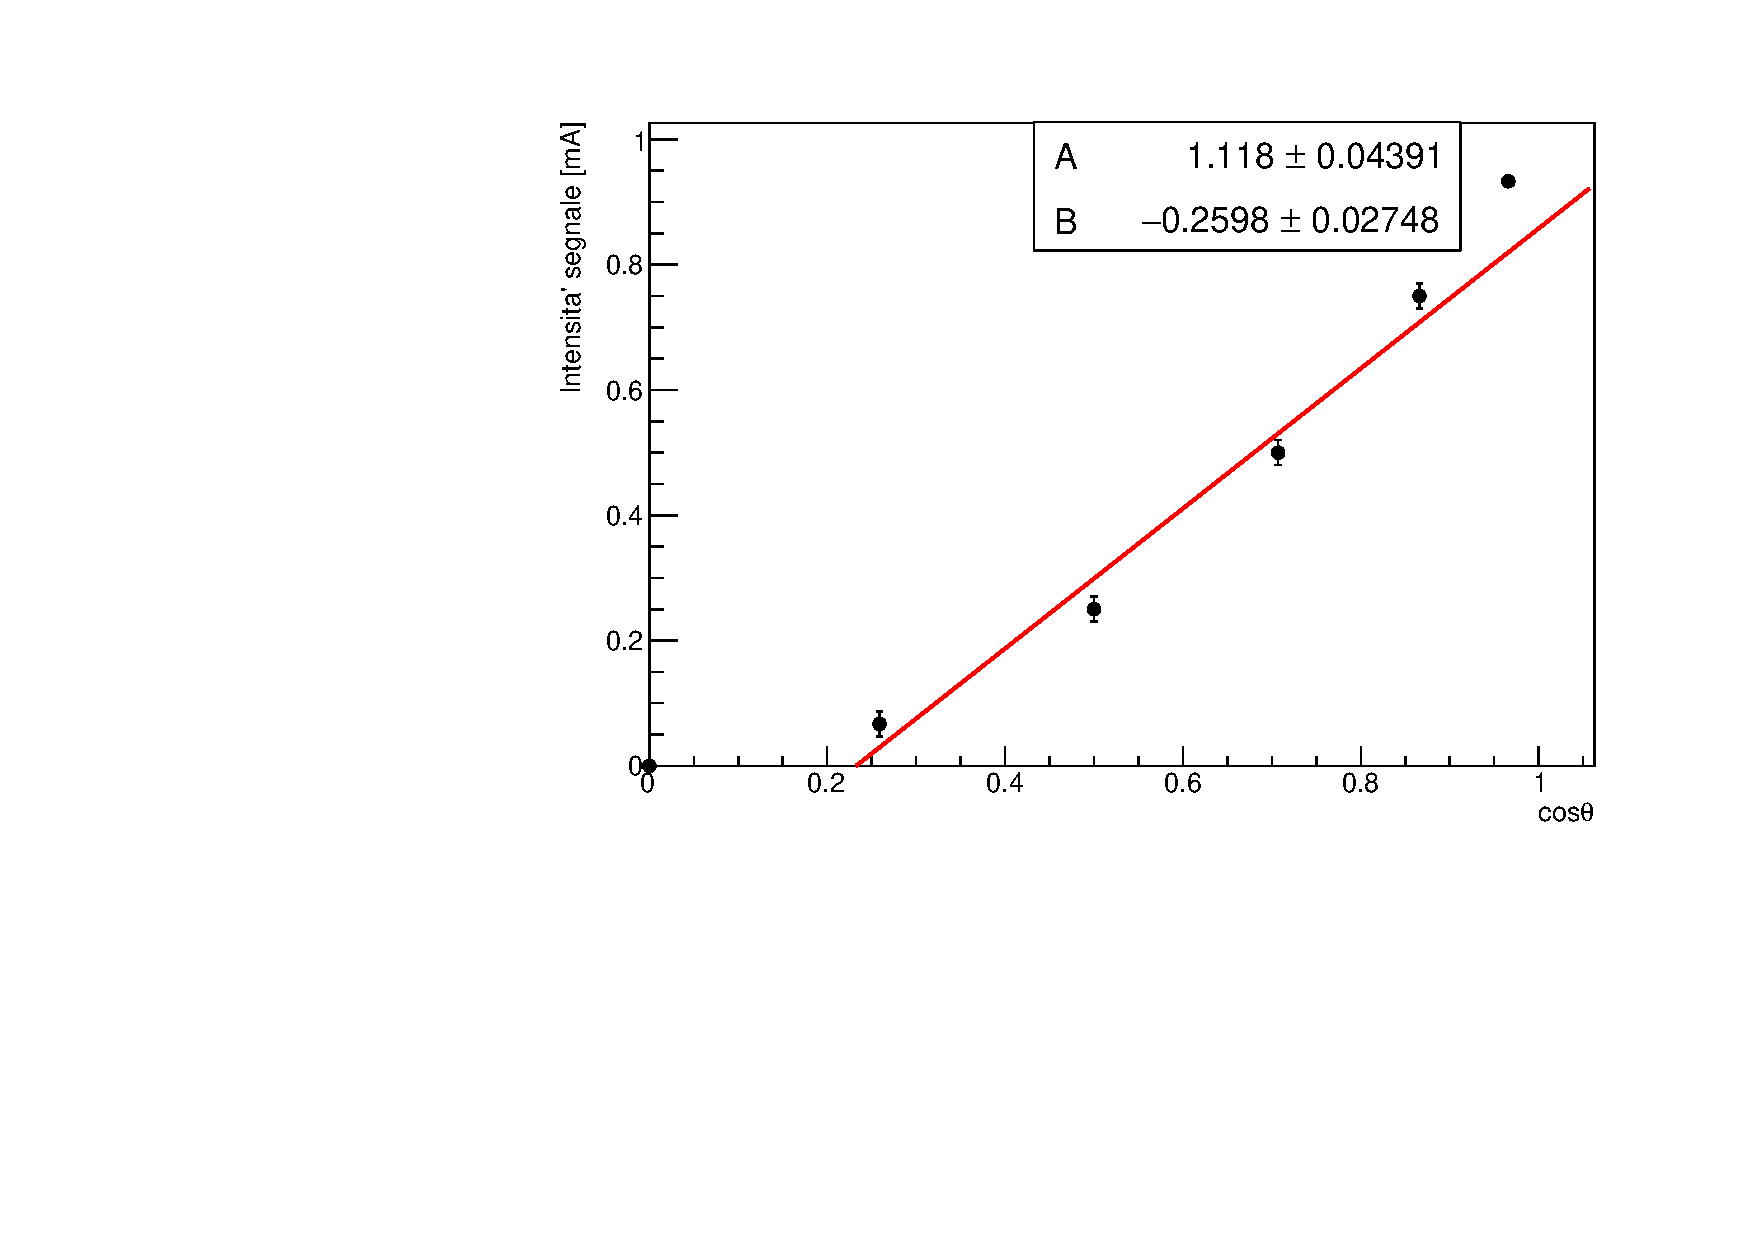
\includegraphics[scale=.5]{Immagini/coseni quadri lineare.pdf} 
    \caption{Interpolazione lineare}
    \label{polatizzazione fit quadratico}
\end{figure}
Abbiamo dimostrato questo mostrando come l'intensità fosse la medesima per angoli positivi e negativi di uguale modulo.

In secondo luogo abbiamo fatto uso di un'interpolazione quadratica che segue la legge di Malus, in grado di descrivere l'imprecisione sulla relazione tra il segnale rilevato e l'effettivo segnale trasmesso. Abbiamo interpolato seguendo 
$$
y=A\cos(\theta) + B(\cos^2\theta)
$$
dove per $y$ si considera il segnale misurato, il grafico è riportato nella Figura \ref{polatizzazione fit}.

\begin{figure}[h!]
    \centering
    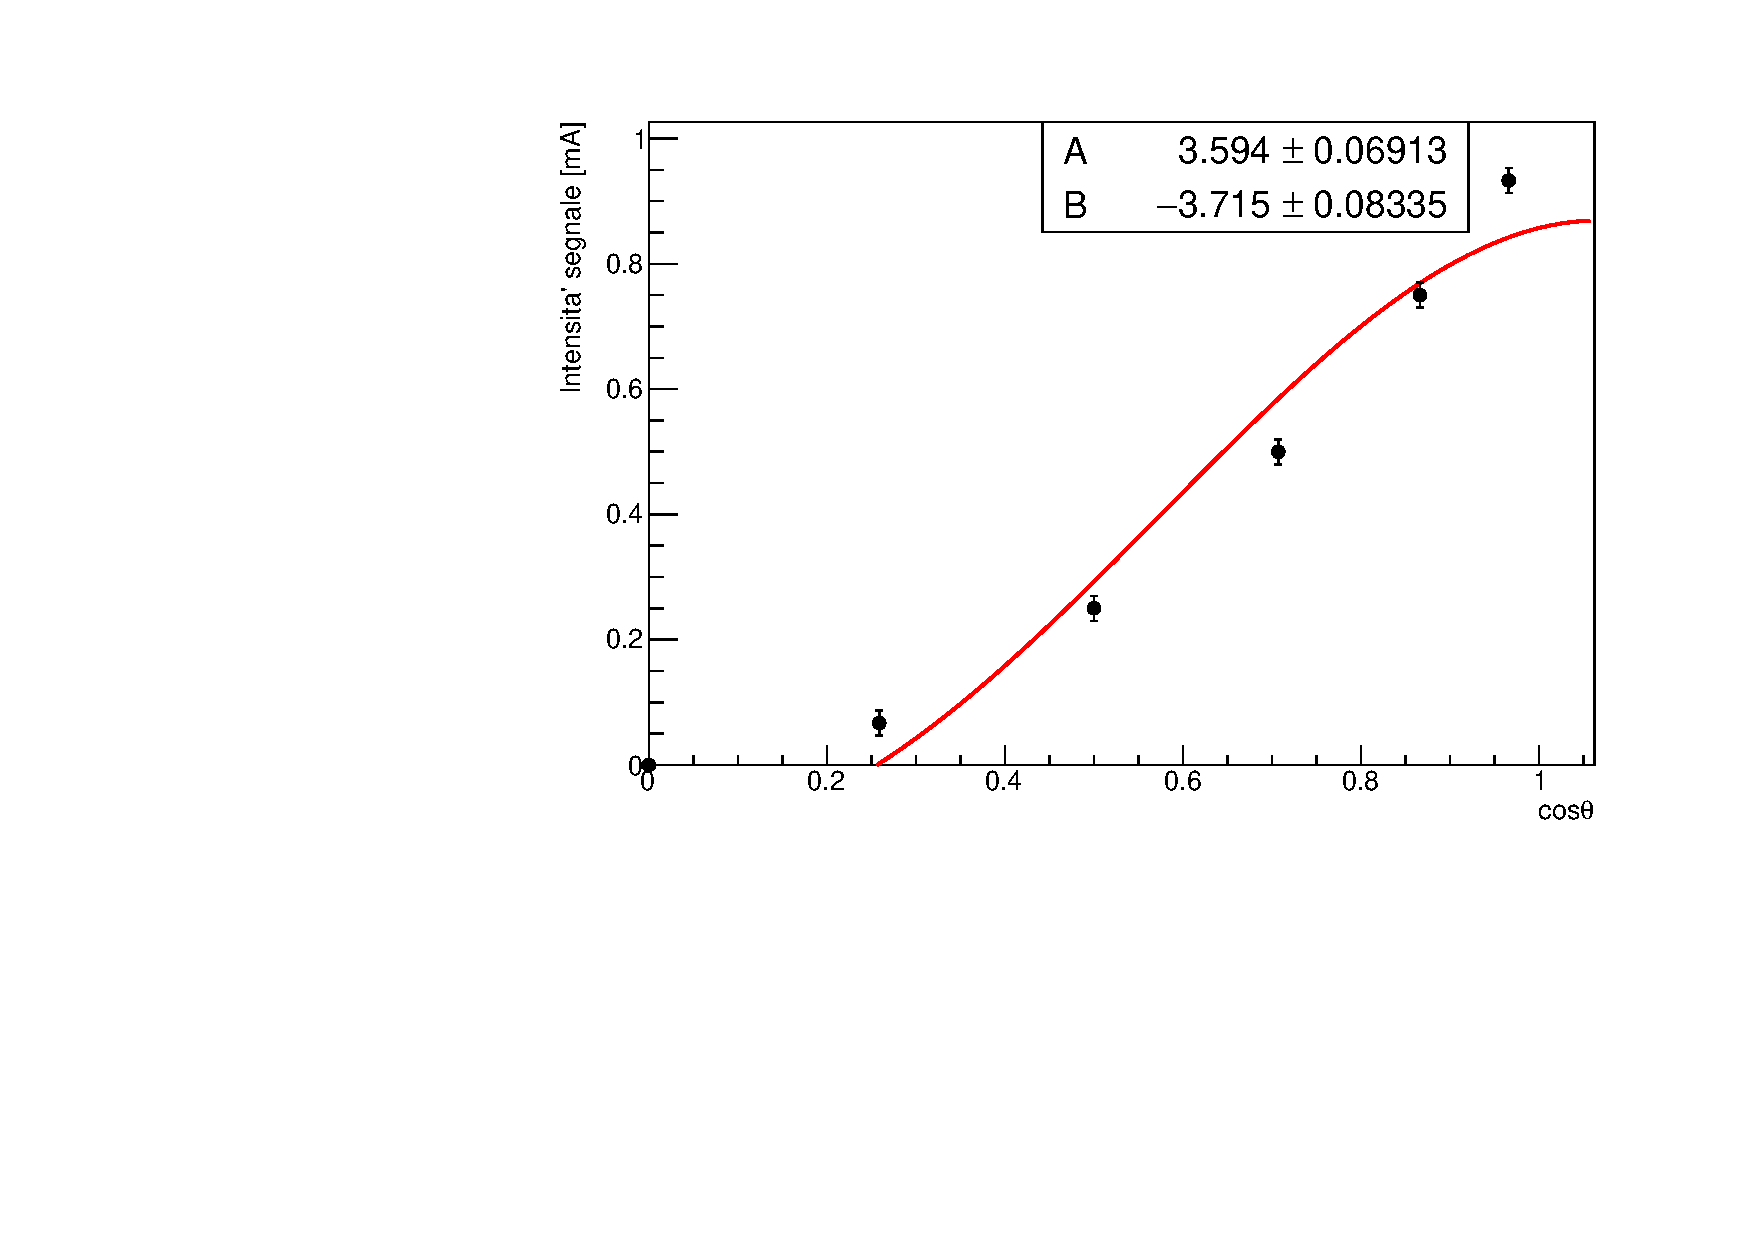
\includegraphics[scale=.5]{Immagini/coseni quadri.pdf}
    \caption{Interpolazione completa}
    \label{polatizzazione fit}
\end{figure}
Non essendo nota la relazione tra il segnale letto sul display dell'Amperometro e il valore medio del campo elettrico nel punto del ricevitore, abbiamo ipotizzato che questo avesse, nel primo caso, una dipendenza lineare dal campo, nel secondo caso, invece, una dipendenza "mista" sia dal campo che dall'intensità.

\section{Angolo di Brewster}
\begin{figure}[h!]
    \centering
    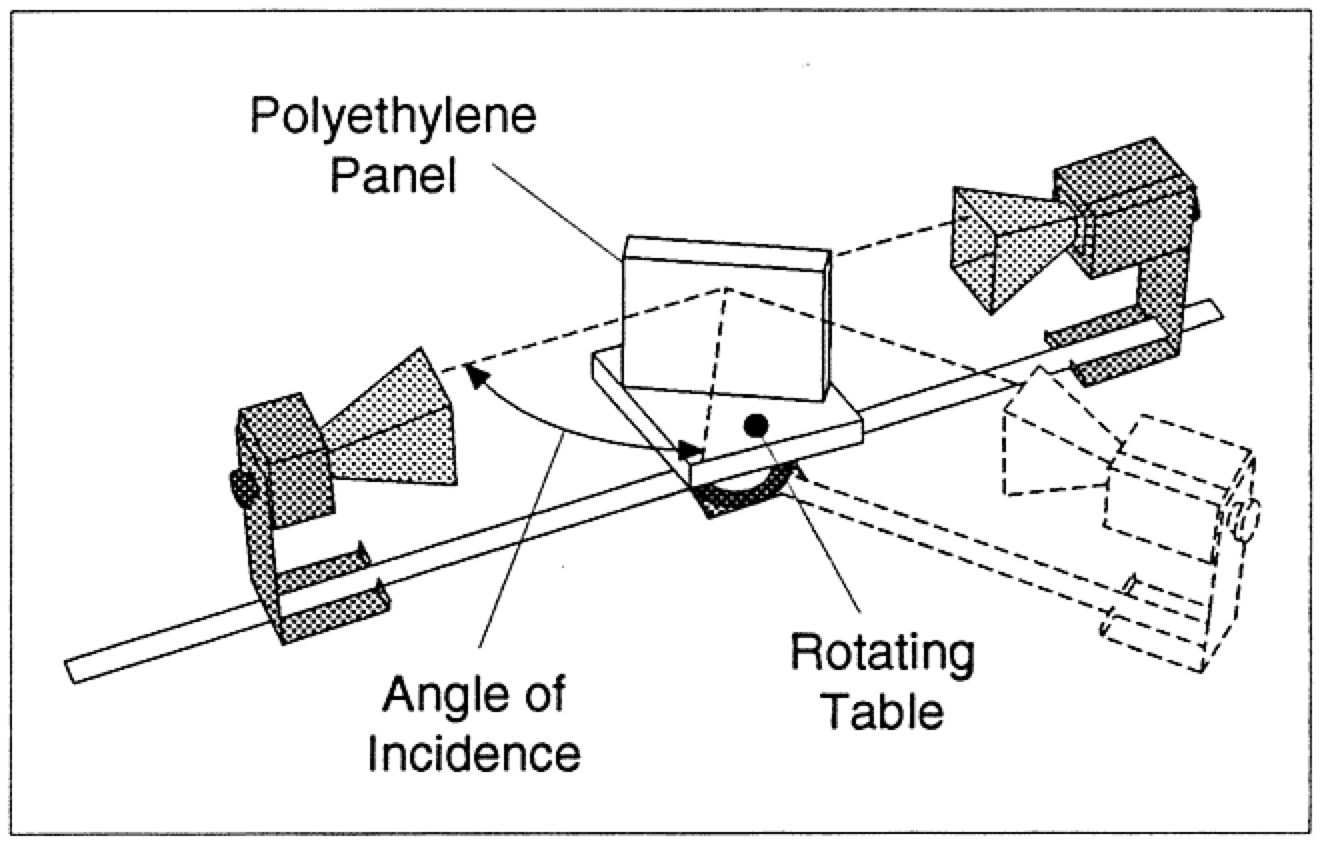
\includegraphics[scale=.3]{Immagini/Schermata 2022-04-07 alle 2.36.29 PM.png}
    \caption{Configurazione dell'apparato sperimentale per la misura dell'angolo di Brewster}
    \label{apparato browser}
\end{figure}

Obiettivo della sezione è stato quello di verificare l'angolo di Brewster.
\noindent
Abbiamo campionato per diversi angoli il valore dell'intensità, con maggiore concentrazione di campionamenti vicino al massimo.
\begin{figure}[h!]
    \centering
    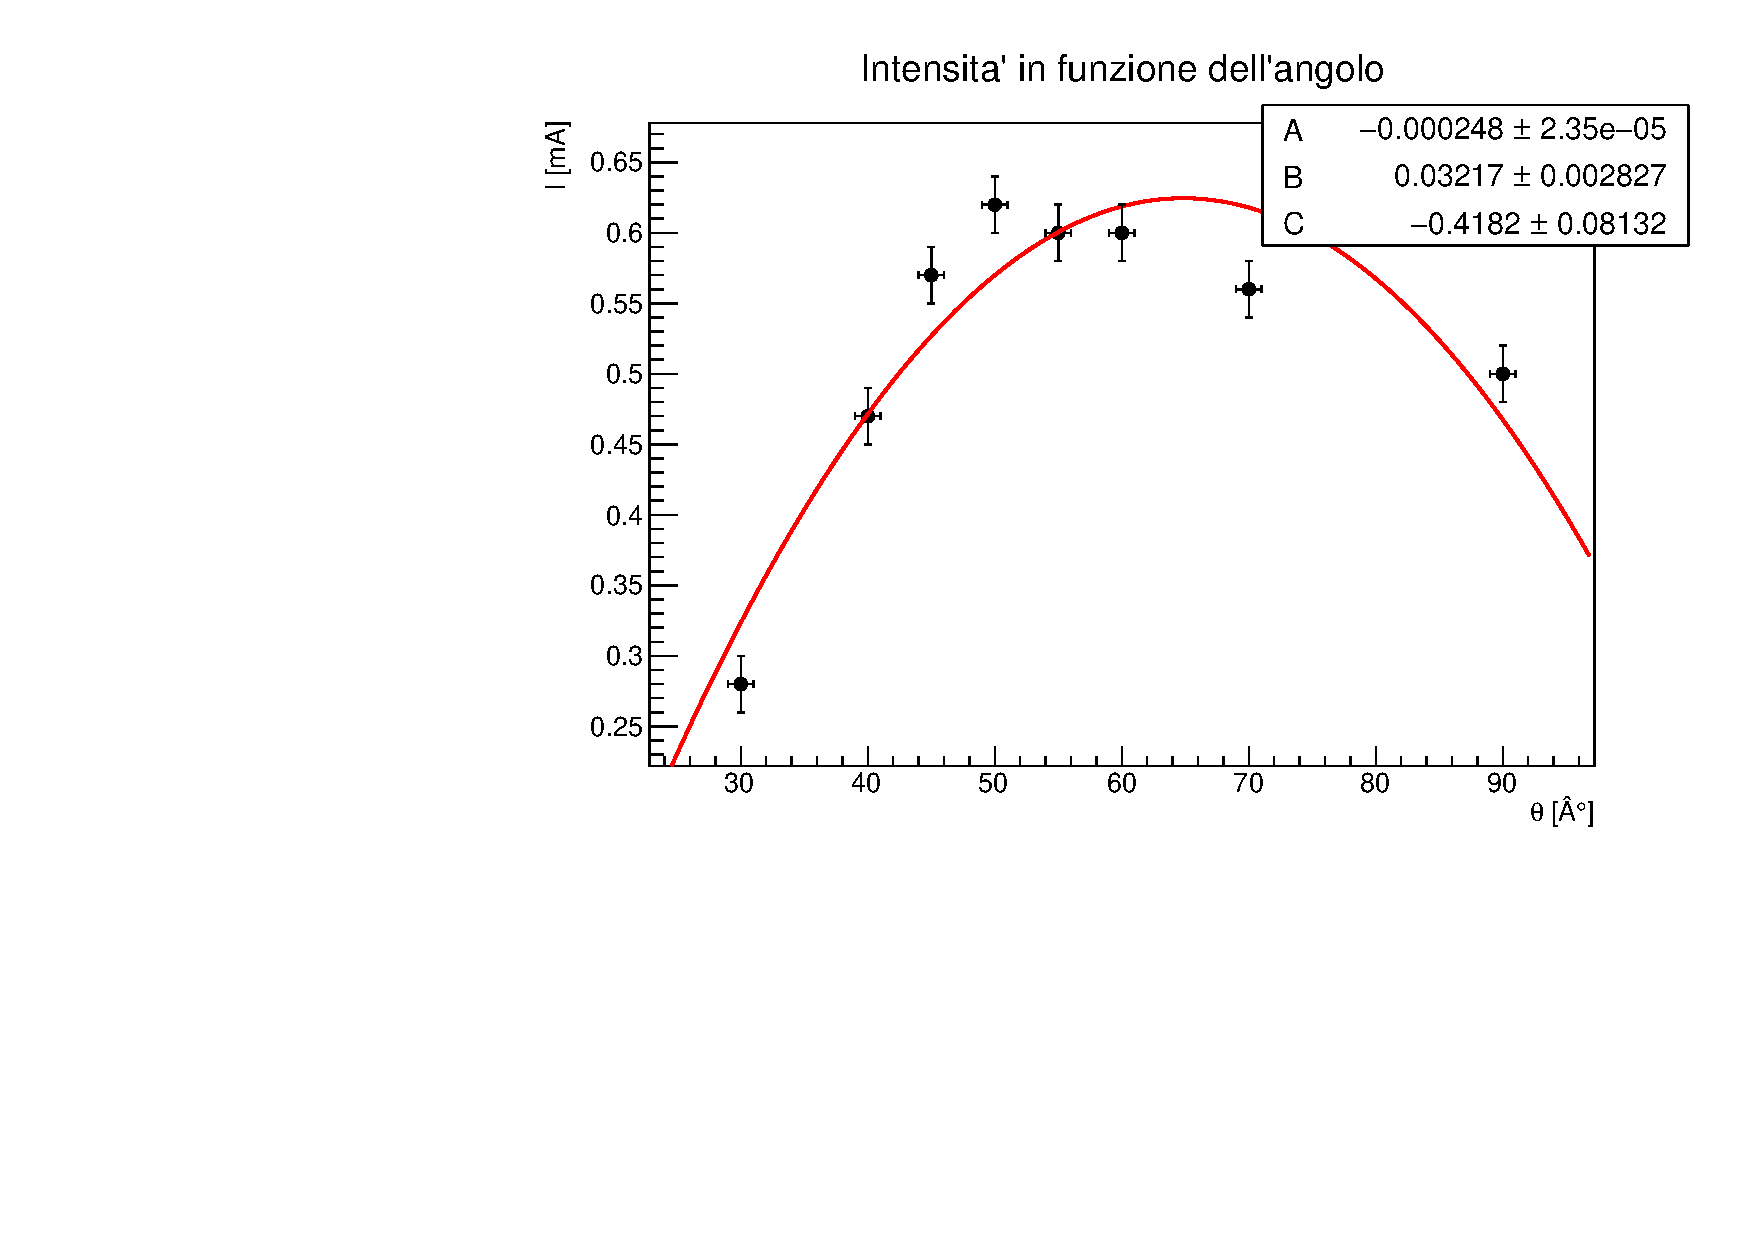
\includegraphics[scale=.5]{Immagini/browser.pdf}
    \caption{}
    \label{}
\end{figure}
Dopo aver interpolato i dati vicino a quest'ultimo, come se questi seguissero una relazione quadratica, abbiamo ricavato il massimo attraverso il calcolo analitico della derivata. Il valore ricavato è $\ang{64}\, 86'$.
Per valutare l'errore abbiamo tenuto conto della correlazione tra $A$ e $B$, calcolando la covarianza tra i due parametri. Covarianza ricavata dalla matrice di covarianza (Eq. \ref{eq 3}) dei tre parametri utilizzati per l'interpolazione.
\begin{equation}
\sigma_{ABC}=
\begin{pmatrix}
5.5232\cdot 10^{-10} & -6.5443\cdot 10^{8} &
1.7909\cdot 10^{-6}\\
\\
-6.5443\cdot 10^{-8} &
7.9896\cdot 10^{-6} & -2.2544\cdot 10^{-4}\\
\\
1.7909\cdot 10^{-6} & -2.2544\cdot 10^{-4} &
6.6125\cdot 10^{-3}\\
\end{pmatrix}
\label{eq 3}
\end{equation}

%La covarianza risulta essere di METTERE VALORE COVARIANZA, l'errore invece di METTERE VALORE ERRORE.
%fare propagazione errore sull'angolo calcolato a mano

\section{Interferenza}
Per analizzare il fenomeno dell'interferenza abbiamo predisposto l'apparato differentemente per due diverse esperienze.

\subsection{Esperienza di Michelson}
In primis abbiamo disposto le lenti e gli specchi come riportato in Figura \ref{michelino}

\begin{figure}[h!]
    \centering
    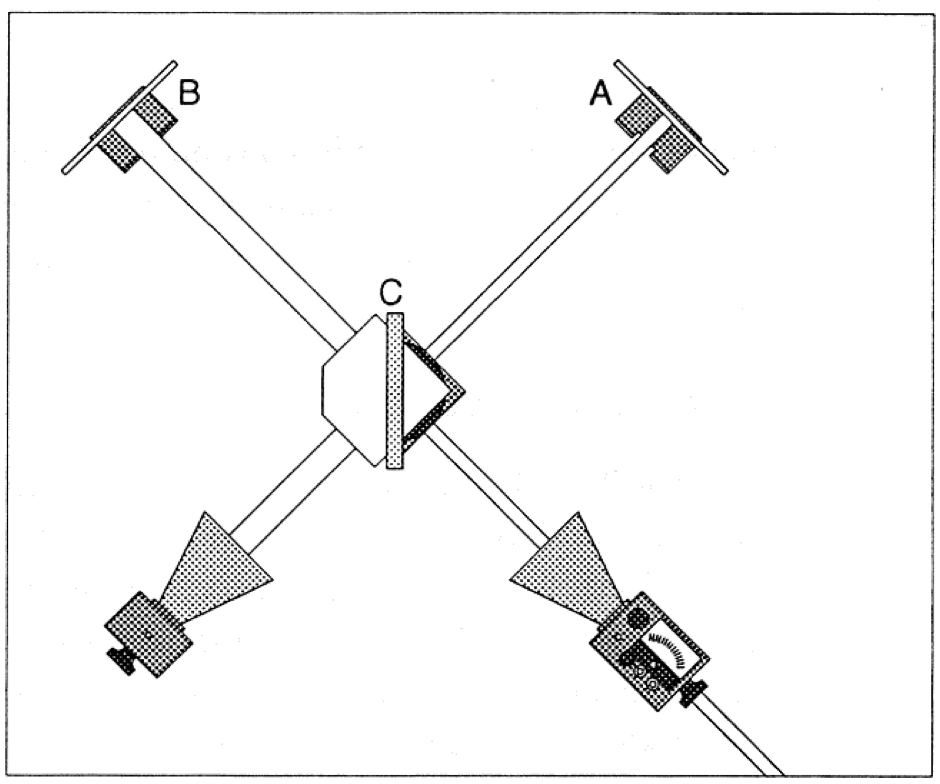
\includegraphics[scale=.35]{Immagini/michelino.png}
    \caption{Configurazione di Michelson}
    \label{michelino}
\end{figure}
\noindent
Mantenendo tutte le componenti fisse, abbiamo proceduto spostando una delle lastre semi-riflettenti con intervalli di $\Delta d = 10 cm$. Dopo aver contato il numero di massimi per tale spostamento, abbiamo calcolato la relativa lunghezza d'onda $\lambda$, utilizzando la seguente relazione:

\begin{equation}
    \lambda=2\dfrac{L_{M1} + \Delta d - L_f}{\Delta N}
\end{equation}
dove $L_{M1}$ indica la posizione iniziale dello specchio mobile e $L_F$ indica la posizione iniziale dello specchio fisso
\noindent
Riportiamo di seguito i valori ricavati:

\begin{table}[h!]
    \centering
    \begin{tabular}{c|cc}
    Numero di massimi & $\lambda$ $(cm)$ & $\sigma_\lambda$ ($cm$)\\
    \hline
6	&	3,33	&0,06\\
6	&	3,33	&0,06\\
7	&	2,86	&0,05\\
7	&	2,86	&0,05\\
7	&	2,86	&0,05\\
7	&	2,86	&0,05\\
7	&	2,86	&0,05\\
7	&	2,86	&0,05\\
8	&	2,50	&0,04\\
7&		2,86&	0,05\\
6	&	3,33	&0,06\\
6&		3,33&	0,06\\
7&		2,86&	0,05\\
7	&	2,86	&0,05\\
7	&	2,86	&0,05\\
7	&	2,86	&0,05\\
7	&	2,86	&0,05\\
\hline\hline
    \end{tabular}
    \caption{Caption}
    \label{tab:my_label}
\end{table}
\noindent
Il valore medio della lunghezza d'onda e il relativo errore, calcolato come media di ogni errore calcolato con il metodo della propagazione degli errori, è di 
$$
\lambda = 2,948 \pm 0,051\, cm
$$
\subsection{Esperienza di Lloyd}
Anche il questo caso lo scopo dell'esperimento è stato quello di determinare la lunghezza d'onda attraverso lo studio del fenomeno dell'interferenza.

Predisposte le componenti come in Figura \ref{loyd} abbiamo cercato di rilevare la posizione dei massimi a partire dal primo. Tale operazione è risultata difficile a causa delle numerose fonti d'incertezze. 

\begin{figure}[h!]
    \centering
    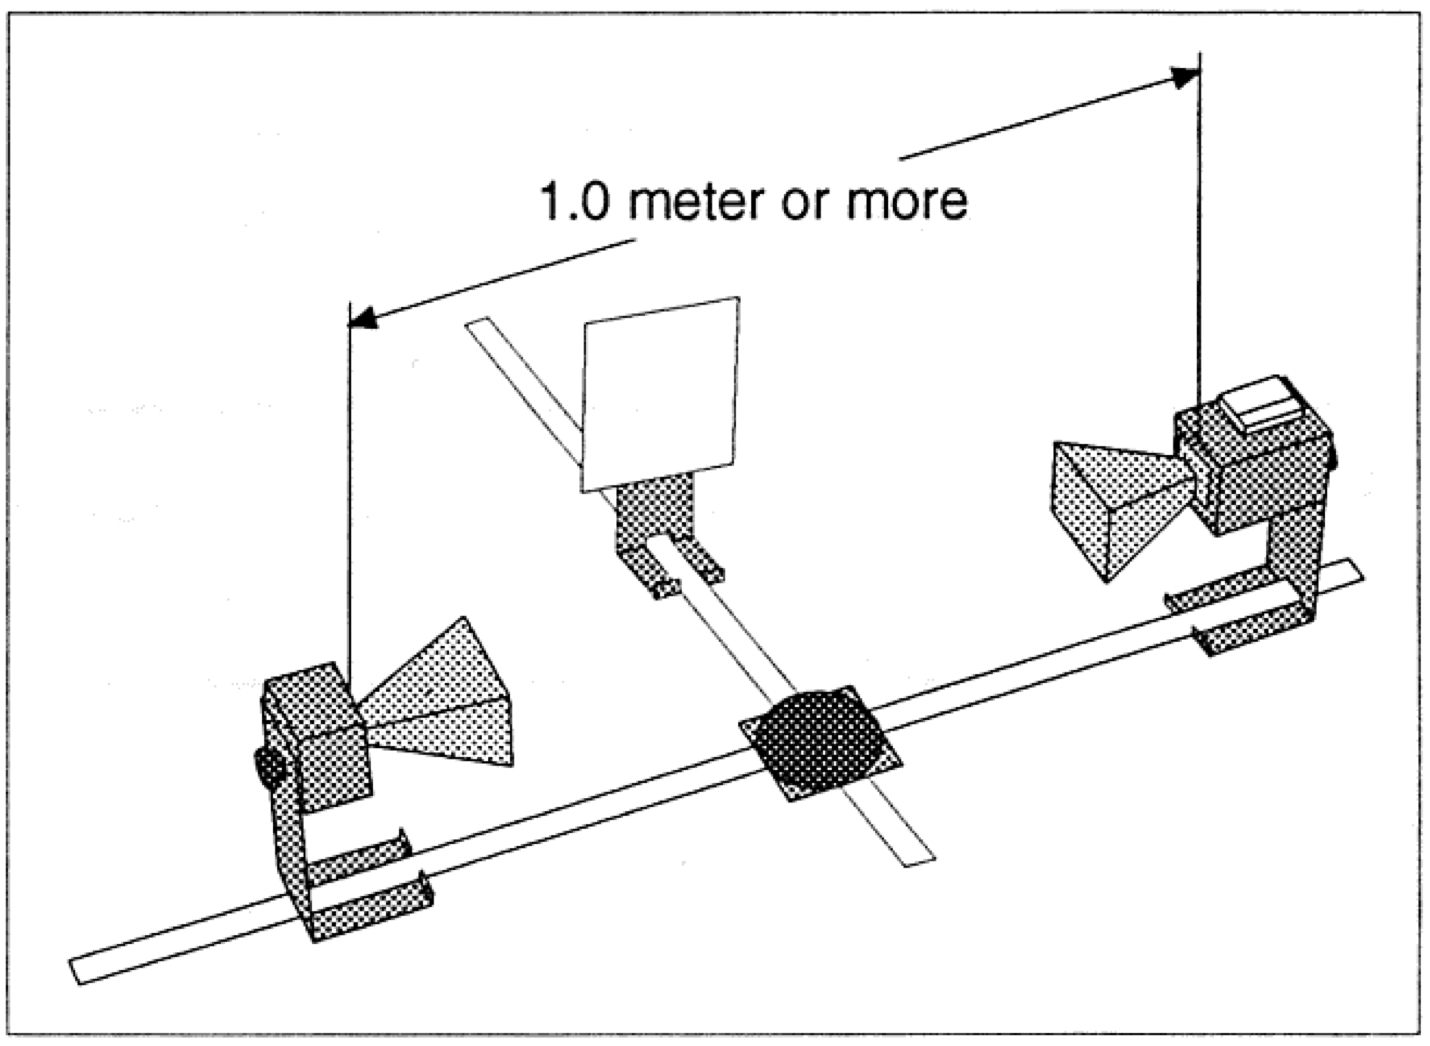
\includegraphics[scale=.35]{Immagini/loid.png}
    \caption{}
    \label{loyd}
\end{figure}
\noindent
I dati raccolti sono i seguenti:
\begin{table}[h!]
    \centering
    \begin{tabular}{ccc}
        Numero del massimo & $d$ $(cm)$ & $\lambda$ $(cm)$ \\
        \hline 
    1&	3,4&1,0	\\
    2&	4,4&5,1	\\
    3&	9,5&2,5	\\
    4&	12&	   4,0 \\
    5&	16&	    8,1\\
    6&	24,1&	\\
\hline\hline
\end{tabular}
\end{table}

E' ben visibile l'errore che traspare dalle misurazioni effettuate, esso verrà discusso nel dettaglio all'interno delle conclusioni.

\section{Conclusioni}
Lo scopo di questa esperienza è stato quello di studiare e verficare relazioni e leggi riguardanti resistenze e diodi. In primo luogo è stata condotta una verifica sulle due configurazioni, quella con il voltmetro e quella con l'amperometro, al fine di analizzare i loro comportamenti rispetto alle configurazioni ideali. Per l'amperometro i risultati ottenuti risultano congruenti con quelli aspettati, cosa che invece non accade con il voltmetro. Crediamo che la causa di ciò possa essere dovuta a due principali fattori. In primis riteniamo possibile che la resistenza scelta, la quale era necessario fosse confrontabile con quella del voltmetro, potrebbe non essere stata tale e che, quindi, l'errore sull'ordine di grandezza potrebbe essere stato causato da quello. Come seconda fonte di errore riconduciamo il fatto che, per identificare le resistenze, ci siamo serviti del tool online menzionato nell'introduzione, i cui valori potrebbero non corrispondere a quelli reali, inserendo quindi un possibile errore sistematico nei nostri risultati. A causa di tale incongruenza, in esperienze che fornivano la possibilità di scegliere la configurazione, abbiamo sempre preferito utilizzare quella con l'amperometro. Lo studio sulla relazione evidenziata da Ohm risulta corretta, nonostante il $\chi^2$ risulti molto bassa. La causa più probabile di questo fenomeno potrebbe essere ricercata in una sottostima degli errori, dovuta al nostro modo di identificare i valori delle resistenze. Nonostante questa possibile fonte di errore, lo studio sul partitore resistivo ha portato risultati congruenti rispetto al nostro studio teorico riguardo alle relazioni sulle resistenze. Infine, anche l'analisi sul diodo risulta congruente rispetto alla relazione ipotizzata, con un $\chi^2$ ridotto di circa 0.82. Riteniamo che l'esperimento potrebbe essere riprodotto con risultati più soddisfacenti se si procedesse a misurare le resistenze in maniera differente. 

\end{document}